\documentclass{tudelft-report}

%% We need to increase the paper size to slightly larger than twice A4 to make
%% room for a front and back cover, including the spine.


\usepackage{fancyhdr}
\usepackage{lipsum}
\usepackage{todonotes}

\usepackage{float}
\usepackage{csquotes}

\usepackage{listings}       % Lstlisting code viewer

\usepackage{longtable}      % Multipage tables

\usepackage{bytefield}

\newcommand{\fakeeighteenbits}[1]{%
    \tiny
    \ifnum#1=1234567890
        #1
    \else
        \ifnum#1<5
            #1%
        \else
            \ifnum#1<13
                $\cdots$%
            \else
                \ifnum#1=13
                    $N-1$
                \else
                    \ifnum#1=14
                        $N$
                    \else
                        \ifnum#1=15
                            $N+1$
                        \else
                            \ifnum#1=16
                                $N+2$
                            \else
                                $N+3$
                            \fi
                        \fi
                    \fi
                \fi
            \fi
        \fi
    \fi
}

\newcommand{\fakeeighteenbitss}[1]{%
    \tiny
    \ifnum#1=1234567890
        #1
    \else
        \ifnum#1<5
            #1%
        \else
            \ifnum#1<13
                $\cdots$%
            \else
                \ifnum#1=13
                    $\cdots$%
                \else
                    \ifnum#1=14
                        $\cdots$%
                    \else
                        \ifnum#1=15
                            $N-2$
                        \else
                            \ifnum#1=16
                                $N-1$
                            \else
                                $N$
                            \fi
                        \fi
                    \fi
                \fi
            \fi
        \fi
    \fi
}

\addtolength{\headheight}{0.9cm} % make more space for the header
\pagestyle{fancyplain} % use fancy for all pages except chapter start
\lfoot{
\includegraphics[height=1.3cm]{figures/colortudelft.png}} % left logo
\rhead{
\includegraphics[height=1.3cm]{figures/projectluna.png}} % right logo
\renewcommand{\headrulewidth}{0pt} % remove rule below header

\setlength\parindent{0pt}       % Do not indent a new paragraph

\def\iic{\texorpdfstring{I$^2$C}{I2C}}  % I2C text format


\definecolor{darkpink}{rgb}{1.0, 0.13, 0.32}


\lstdefinestyle{DOS}
{
    backgroundcolor=\color{black},
    basicstyle=\scriptsize\color{white}\ttfamily
}


\begin{document}
%% Use Roman numerals for the page numbers of the title pages and table of
%% contents.
% \frontmatter

%% Uncomment following 19 lines for a cover with a picture on the lower half only
\title[tudelft-white]{Bus Manager}
\subtitle[tudelft-cyan]{Lunar Zebro}
\author[tudelft-white]{Software Department}
\affiliation{-}
\coverimage{figures/page1background.png}
\titleoffsetx{2cm}
\titleoffsety{8cm}
\afiloffsetx{1cm}
\afiloffsety{18cm}
\covertext[tudelft-white]{
    \textbf{Cover Text} \\
    possibly \\
    spanning
    multiple
    lines
    \vfill
    ISBN 000-00-0000-000-0
}
\setpagecolor{black}
\makecover



%
%% Include an optional title page.
\begin{titlepage}


\begin{center}

%% Insert the TU Delft logo at the bottom of the page.

%% Print the title in cyan.
{\makeatletter
\largetitlestyle\fontsize{64}{94}\selectfont\@title
%\largetitlestyle\color{tudelft-cyan}\Huge\@title
\makeatother}

%% Print the optional subtitle in black.
{\makeatletter
\ifx\@subtitle\undefined\else
    \bigskip
   {\tudsffamily\fontsize{22}{32}\selectfont\@subtitle}
    %\titlefont\titleshape\LARGE\@subtitle
\fi
\makeatother}

\bigskip
\bigskip

by
%door

\bigskip
\bigskip

%% Print the name of the author.
{\makeatletter
%\largetitlefont\Large\bfseries\@author
\largetitlestyle\fontsize{26}{26}\selectfont\@author
\makeatother}

\bigskip
\bigskip

in partial fulfilment of the requirements for documentation for:
%ter verkrijging van de graad van Master of Science

TU Delft, The Netherlands
%aan de Technische Universiteit Delft,

%to be defended publicly on Tuesday January 1, 2013 at 10:00 AM.
%in het openbaar de verdedigen op dinsdag 1 januari om 10:00 uur.

\vfill

\begin{tabular}{lll}
    Project Director: & prof. dr. ir. C. J. M. Verhoeven, & TU Delft \\
    System Engineer: & Pranav Gurumallappa, & TU Delft \\
    Operations Manager: & Maneesh Verma, & TU Delft \\
%    Project duration: & \multicolumn{2}{l}{March 1, 2012 -- January 1, 2013} \\
    Head of Software: & dr. A. Noroozi, & TU Delft \\
    Vice Head of Software: & Y. Klaassens, & TU Delft \\
\end{tabular}
%% Only include the following lines if confidentiality is applicable.

\bigskip
\bigskip
\emph{This document is confidential and cannot be made public unless a written permission has been obtained from project director.
}
%\emph{Op dit verslag is geheimhouding van toepassing tot en met 31 december 2013.}

\bigskip
\bigskip
%An electronic version of this thesis is available at %\url{http://repository.tudelft.nl/}.
%\\[1cm]

%\centering{
\includegraphics{cover/logo_black}}


\end{center}

\begin{tikzpicture}[remember picture, overlay]
    \node at (current page.south)[anchor=south,inner sep=0pt]{
        
\includegraphics{cover/logo_black}
    };
\end{tikzpicture}

\end{titlepage}


\tableofcontents

%% Use Arabic numerals for the page numbers of the chapters.
% \mainmatter

\chapter{Introduction}
Because RS485 is a half-duplex protocol, software on both ends of the physical data line should follow the same set of rules defined in the protocol and Message Format (see Chapter \ref{ch:message_format}). The Bus Manager is responsible for transferring commands and data between subsystems while adhering to this format.
This implies checking for CRC errors and sending a retransmission request or NACK when it needs to do so.
The Bus Manager acts between the Application Layer and the Physical Layer of the OSI model.

Figure \ref{fig:rs485_diagram} shows that there are 5 different RS485 buses inside the rover.
The Bus Manager also prevents any race condition on its assigned bus and makes sure that multiple apps cannot communicate with their subsystem at the same time.
\todo[inline]{Not sure about this yet}

\begin{figure}[H]
    \centering
    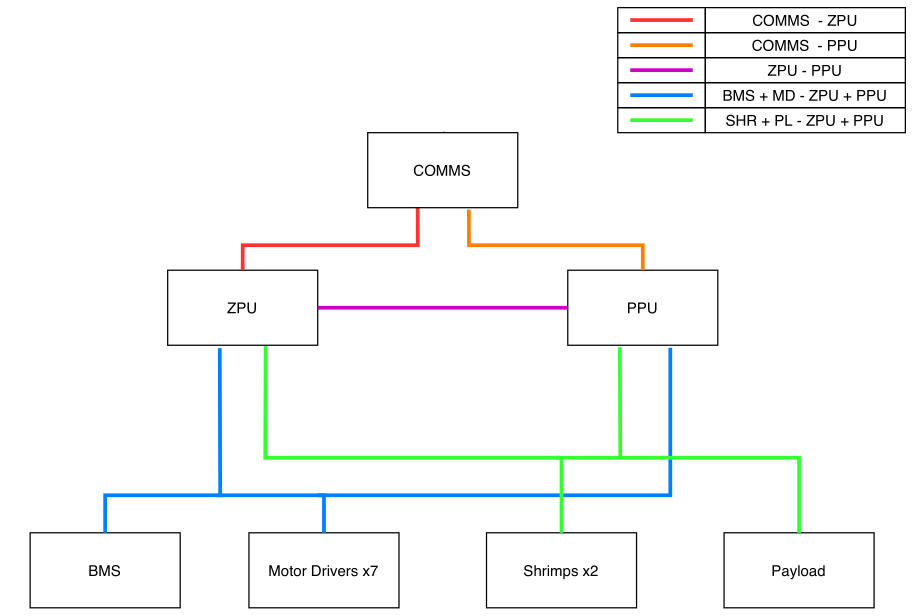
\includegraphics[scale=0.4]{figures/RS485_connections.png}
    \caption{Schematic view of the physical RS485 busses layout}
    \label{fig:rs485_diagram}
\end{figure}


\newpage


It is a bit awkward and impractical to uniquely identify RS485 buses based on the colours used in Figure \ref{fig:rs485_diagram}.
This is why we map the colours of Figure \ref{fig:rs485_diagram} to a unique bus name and number.
Table \ref{tab:buslegend} shows this mapping.
From now on in this document as well as in code, we will refer to bus names rather than bus colours.

\definecolor{amethyst}{rgb}{0.6, 0.4, 0.8}
\definecolor{bleudefrance}{rgb}{0.19, 0.55, 0.91}

\begin{longtable}{| p{0.1\textwidth} | p{0.15\textwidth} | }
    \hline
    \textcolor{red}{Bus name} & \textcolor{red}{Bus colour} \\
    \hline
    Bus0 & 
\begin{tikzpicture} \draw[line width=1mm, color=red] (0,0) -- (2,0); \end{tikzpicture} \\
    \hline
    Bus1 & 
\begin{tikzpicture} \draw[line width=1mm, color=orange] (0,0) -- (2,0); \end{tikzpicture} \\
    \hline
    Bus2 & \begin{tikzpicture} \draw[line width=1mm, color=amethyst] (0,0) -- (2,0); \end{tikzpicture} \\
    \hline
    Bus3 & \begin{tikzpicture} \draw[line width=1mm, color=bleudefrance] (0,0) -- (2,0); \end{tikzpicture} \\
    \hline
    Bus4 & 
\begin{tikzpicture} \draw[line width=1mm, color=green] (0,0) -- (2,0); \end{tikzpicture} \\
    \hline

    \caption{Bus legend mapping bus names to colours}
    \label{tab:buslegend}
\end{longtable}


\section{Background information and History}

\subsection{First version (1.0)}
Bus Manager is a concept that was first introduced in February 2021 as part of Max' thesis \cite{comms_thesis}.
Between February 2021 and August of 2021, the foundational layer of Bus Manager was laid which includes, but is not limited to, the Message Format.
Unit tests have shown that this first revision of Bus Manager used to work.

\subsection{Second version (2.0)}
In the second revision of Bus Manager, a few modifications have been made.
One of these changes is, for instance, that the Bus Manager won't send an initial message to request if an $x$ amount of bytes are available for the receiver to receive. Instead, it will just send the command which includes the length as part of the Message Format.
\todo[inline]{Clear up this sentence}
\par The second revision also uses a semaphore to synchronise bus access between bus managers, because the idea was for each subsystem app to have its own bus manager.

\subsection{Third version (2.1)}
The third version of the Bus Manager uses a more centralised approach. The Bus Managers live on the OBC in their own app, which coordinates bus access for all buses. Apps need to communicate with the Bus Managers via inter-thread communication. This avoids the need for using shared semaphores and decreases the dependencies between the subsystem apps. For further information about the design, see Chapter \ref{ch:design}.


\section{List of features of Bus Manager 2.1}

Now that the reader is aware of the overall functionality of the Bus Manager, we can list a set of features that characterises Bus Manager 2.1 (subject to change).

\begin{itemize}

    \item{\textbf{Instances}. Each bus has a separate instance of the Bus Manager that manages the access to that bus. Avoids the need for a more complex solution for all buses.}

    \item{\textbf{Timeout}. When a Bus Manager sends any type of message it waits for a response. A configurable timeout limit can be set to signal an error if the response is not received within that limit. }

    \item{\textbf{Retries}. When too many timeouts have happened and \textbf{<tbd>} retries are exceeded, then the application layer of this particular Bus Manager is informed about the failure.}

    \item{\textbf{Portability}. Because of the extensive use of Bus Manager both on the masters (OBC, PPU) and slaves (subsystems), it is of extra interest to design and implement Bus Mananger in such a way that it is easy to port over to subsystems which run different hardware architectures. Reimplementing it means that subsystem designers need to be fully aware of the protocol- and Message Format and this is a source of error and requires extra testing and validating. Bus Manager should be easily portable and be abstract in nature.}

    \item{\textbf{Sustainability}. Bus Manager shall comply to the Lunar Zebro Software guidelines. These include, but are not limited to: the code style guide and GoogleTest Unit Tests. The Git repository follows the same skeleton as all the other software modules.}

\end{itemize}


%\chapter{Failure Modes and Effect Analysis (FMEA)}
%\todo[inline]{Needs updating!}
%This chapter focuses on the different failure modes that can occur when sending and receiving messages, their effects and possible mitigation strategies.
%
%\begin{longtable}{|p{1.8cm}|p{2.5cm}|p{2.5cm}|p{2.5cm}|p{2.5cm}|p{2.5cm}|}
%	\hline
%	\textbf{Function} & \textbf{Failure Mode} & \textbf{Cause} & \textbf{Likelihood} & \textbf{Effect} & \textbf{Mitigation} \\
%	\hline
%	Initialisation & Already initialised & init called twice & & Initialisation fails & No mitigation necessary. \\
%		\hline
%		& Open semaphore fail & No permission OR too many open files OR insufficient memory & & Unable to access bus for all apps & \todo[inline]{TBD} \\
%		\hline
%		& Claim semaphore fail & Semaphore was deleted OR other app still has semaphore & & Unable to access bus & Retry the claim TBD times. \todo[inline]{What if retries fail?}\\
%		\hline
%		& Release semaphore fail & Semaphore was deleted & & Unable to access bus for all apps & \todo[inline]{TBD} \\
%		\hline
%		& Serial not configured & TRON did not configure serial & & Unable to access bus for all apps & \todo[inline]{TBD} \\
%		\hline
%	Destruction & Close semaphore fail & Invalid file descriptor & & Semaphore is not closed & \todo[inline]{TBD} \\
%		\hline
%		& Unlink semaphore fail & No permission OR semaphore was deleted OR semaphore was never created & & Semaphore is not deleted & If error is EACCESS, we might need to reboot. \todo[inline]{TBD} \\
%		\hline
%		& Close serial bus fail & Serial not configured & & No effect & No mitigation needed \\
%		\hline
%	Interfacing & Claim semaphore fail & Semaphore was deleted OR other app still has semaphore & & Unable to access bus & Retry the claim TBD times. \todo[inline]{What if retries fail?} \\
%		\hline
%		& Release semaphore fail & Semaphore was deleted & & Unable to access bus for all apps & \todo[inline]{TBD} \\
%		\hline
%	Reading & Reading timeout & Subsystem not functioning OR bus not functioning & & No communication with subsystem & Retry TBD times. If all retries fail, forward error to app. \\
%		\hline
%		& Read blocks indefinitely & Continuous stream of data & & No communication with subsystem & \todo[inline]{TBD} \\
%		\hline
%		& Reading error & Serial not configured & & Unable to access bus for all apps & \todo[inline]{TBD} \\
%		\hline
%		& Bitflip in message & Radiation hit & & Message is invalid & Use a CRC to detect an invalid message. \\
%		\hline
%		& Bitflip with valid CRC & Radiation hit twice & & Invalid message perceived as valid & Delegate handling to the app. \\
%		\hline
%		& MD field is always 1 & Invalid subsystem firmware & & Wait for a message that never comes & Use read timeout to catch this. \todo[inline]{Maybe add expected amount of messages?} \\
%		\hline
%		& CRC is always invalid & Invalid subsystem firmware & & Valid message perceived as invalid &  \todo[inline]{TBD}\\
%		\hline
%		& SN/NESN are always incorrect & Invalid subsystem firmware & & ACK'd message perceived as NACK & \todo[inline]{TBD} \\
%		\hline
%	Writing & Writing error & Serial not configured OR no free space OR invalid device file & & Unable to access bus & \todo[inline]{TBD} \\
%		\hline
%		& Message never arrives & Subsystem not functioning OR bus not functioning & & No communication with subsystem & Use the read timeout for this. Delegate error handling to app. \\
%		\hline
%		& \# bytes written is less than desired & & & Subsystem does not receive all bytes & \todo[inline]{TBD} \\
%		\hline
%\end{longtable}

\chapter{Design}
\label{ch:design}

\section{General design}
The high-level functionality of the bus manager is displayed in Table \ref{tab:functionality}.

\begin{table}[H]
\centering
\begin{tabular}{|p{2cm}|p{8cm}|}
	\hline
	\textbf{Code} & \textbf{Function}\\\hline
	BM\_F1 & Configure RS-485 buses\\\hline
	BM\_F2 & Manage access to RS-485 buses \todo[inline]{Not sure}\\\hline
	BM\_F3 & Translate subsystem commands to serial bus messages and vice versa using the message protocol \\\hline
	BM\_F4 & Check correctness of the received messages \\\hline
\end{tabular}
\caption{High-level functions of the bus manager.}
\label{tab:functionality}
\end{table}

When the rover starts up, the bus managers configure and initialise the physical buses once (\textbf{BM\_F1}). The programmer can use the public interfaces to send messages to the bus and receive messages from the bus (BM\_F3). The bus manager checks if all received messages are correct and if they are not, it retries or signals an error (BM\_F4).

\section{Detailed design}
This section describes the design decisions in more detail.
\subsection{Initialisation}
\label{sec:initialisation}
There are a total of 5 bus manager instances on the OBC, one for each bus. In addition, each subsystem has its own bus manager instance running in its firmware. Each instance is initialised only once. This initialisation configures the serial bus using the correct settings. This configuration can be different for different devices. The bus manager abstracts away from this configuration so the programmer needs to implement this lower-level functionality!

\subsection{Interfacing (read/write)}
\label{sec:interfacing}
A diagram of the steps involved in the interfacing process can be found in Figure \ref{fig:read_write_design}. The bus managers on the OBC exclusively use this functionality. The subsystems also use it, but only after first reading from the bus (see Section \ref{sec:subsystem_interfacing}).
\par After writing each packet, the bus manager reads the responses. These can be either an ACK or a REPLY. For each REPLY received, the bus manager sends an ACK response.

\begin{figure}[H]
	\centering
	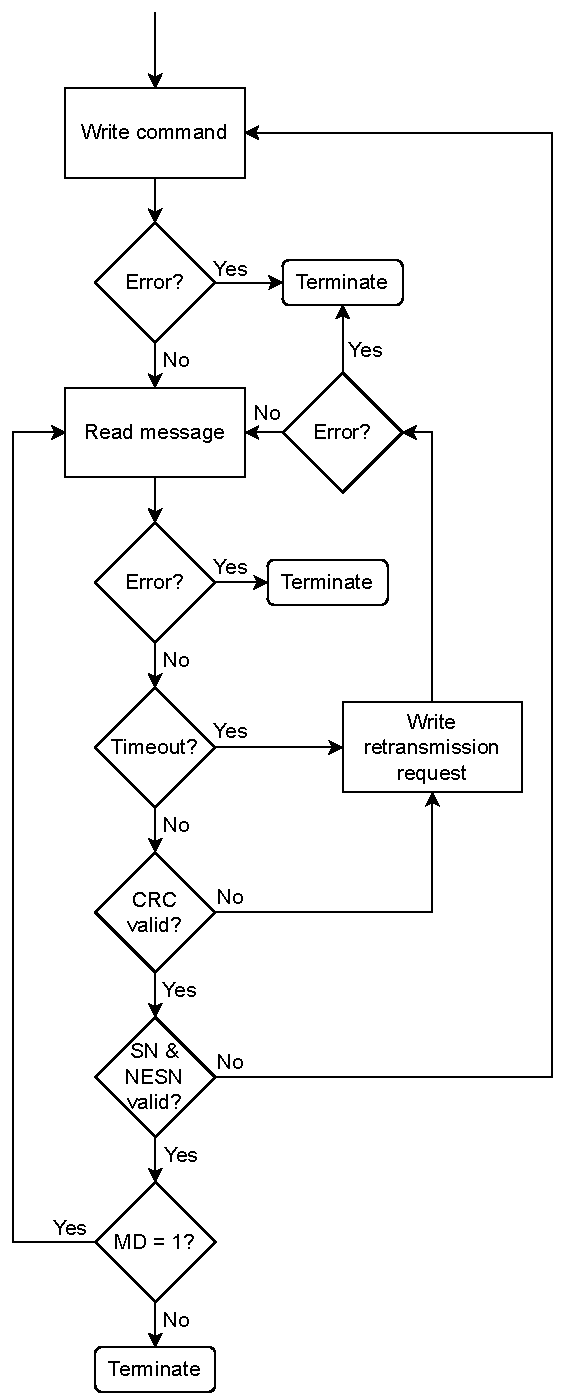
\includegraphics[width=0.4\textwidth]{figures/Bus_manager_diagram.pdf}
    \caption{High-level design diagram for serial writing using the bus manager}
    \label{fig:read_write_design}
\end{figure}

\begin{enumerate}
	\item \textbf{Write} the command to the serial bus.
	\item \textbf{Check for errors} after writing.
	\item \textbf{Read} the next incoming message.
	\item \textbf{Check for errors} after reading:
	\begin{itemize}
		\item Check for valid CRC
		\item Check for read timeout
	\end{itemize}
	\item \textbf{Send a retransmission request} and go to step 3 if an error occurred.
	\item \textbf{Check SN/NESN} message fields.
	\item \textbf{Retransmit the command} and go to step 3 if SN and/or NESN are invalid.
	\item \textbf{Send an ACK} packet to the serial bus.
	\item Go to step 3 if the MD field is set to 1.
\end{enumerate}

\subsection{Subsystem interfacing}
\label{sec:subsystem_interfacing}
The subsystem interfaces a bit differently, since it actively needs to listen for commands from the OBC or PPU. So it first reads from the bus, then uses the interfacing procedure described in Section \ref{sec:interfacing}.

%The overall design for interfacing between the host and controller is given in Figure \ref{fig:read_write_design}.
%We explain each step in a bit more detail below:
%\begin{itemize}
%	\item \textbf{Claim semaphore}: semaphore is claimed at the start of the sequence so response messages are not read by a different bus manager. We need to keep the semaphore until termination for the same reason: we don't want a bus manager to interrupt the message sequence. It is also crucial that the read/write operation is not interrupted, so we need to define a critical region \todo[inline]{How do we make sure the task is not preempted?}.
%	Lastly, we need to use a timeout for the semaphore claim. If a bus manager infinitely loops for some reason, we can never claim the semaphore and the whole system would lock up.
%	\item \textbf{Write message}: write a message to the serial bus and propagate any errors.
%	\item \textbf{Read message}: read a message from the serial bus. The read has a certain timeout specified by the programmer, which can be different for different messages. If the read times out an error is raised and the interfacing is terminated.
%	\item \textbf{Check CRC}: CRC is calculated over the payload in the response message and compared to the CRC inside the response message. If they do not match, the bus manager sends a retransmission request to the destination the response messasge came from. This is done until the bus manager runs out of retries or until the CRC is correct.
%	\item \textbf{Check ACK}: SN and NESN are checked to see if the request message was acknowledged or not. If it was not, the request message is retransmitted. This is done until the message is acknowledged or when the bus manager runs out of retries.
%	\item \textbf{Send ACK}: If everything in the message is correct, the bus manager sends an acknowledgement to the subsystem to indicate it received the message.
%	\item \textbf{Check MD}: if the MD bit is set, more data is on the way and we should read another message. This is done until MD is not set anymore.
%	\todo[inline]{Should we put a limit on the MD set? Because if it is always set you enter an infinite loop.}
%\end{itemize}

%\begin{figure}[h]
%	\centering
%	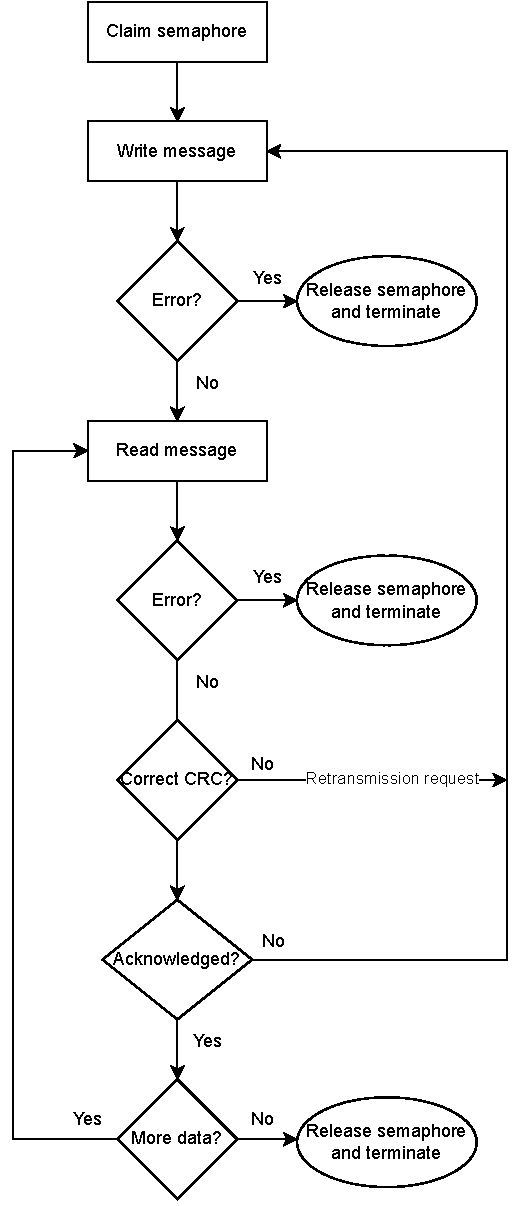
\includegraphics[width=0.3\textwidth]{figures/bus-manager-functional.drawio.pdf}
%    \caption{High-level design diagram for serial reading and writing using the bus manager}
%    \label{fig:read_write_design}
%\end{figure}


%\chapter{Implementation}

%\section{\texttt{Bus\_manager\_t} class}
%Each app will have its own \texttt{Bus\_manager\_t} instance to interface with its subsystem. The bus manager is used for reading and writing from and to one of the 5 serial buses that the OBC has access to. It is important to note that the \texttt{Bus\_manager\_t} class does NOT represent a bus, but merely a class that abstracts from reading and writing and that locks the bus from multiple accesses.
%\par Each of the buses have the following attributes. All of these are implemented as static arrays in the \texttt{Bus\_manager\_t} class.
%\begin{itemize}
	%\item \textbf{Named semaphore}: used to lock the bus to prevent multiple apps accessing the same bus at the same time.
	%\item \textbf{File descriptor}: used to read from and write to the bus. Must be locked using the semaphore before use.
	%\item \textbf{Initialisation variable}: used to indicate if the bus was initialised or not.
	%\item \textbf{State}: bus state. Not sure what this is used for yet.
%\end{itemize}

%\section{CRC calculation}
%We explain each step in a bit more detail below:
%\begin{itemize}
%	\item \textbf{Claim semaphore}: semaphore is claimed at the start of the %sequence so response messages are not read by a different bus manager. We need to keep the semaphore until termination for the same reason: we don't want a bus manager to interrupt the message sequence.
%	\item \textbf{Write message}: write a message to the serial bus and propagate any errors.
%	\item \textbf{Read message}: read a message from the serial bus. The read has a certain timeout specified by the programmer, which can be different for different messages. If the read times out an error is raised and the interfacing is terminated.
%	\item \textbf{Check CRC}: CRC is calculated over the payload in the response message and compared to the CRC inside the response message. If they do not match, the bus manager sends a retransmission request to the destination the response messasge came from.
%	\item \textbf{Check ACK}: SN and NESN are checked to see if the request message was acknowledged or not. If it was not, the request message is retransmitted. This is done until the message is acknowledged or when the bus manager runs out of retries.
%	\item \textbf{Check MD}: if the MD bit is set, more data is on the way and we should read another message. This is done until MD is not set anymore.
%	\todo[inline]{Should we put a limit on the MD set? Because if it is always set you enter an infinite loop.}
%\end{itemize}


\chapter{Implementation}
The implementation consists of two classes.
\begin{itemize}
	\item \texttt{Packet\_t} class: represents a message protocol packet.
	\item \texttt{Bus\_manager\_t} class: represents a bus manager for a single bus.
\end{itemize}
The bus manager class uses the packet class extensively to form packets for writing to the serial bus. Both classes are discussed below in more detail.

\section{\texttt{Packet\_t} class}
The packet class has the same instance variables as the fields of the messages that we use in the messaging protocol:
\begin{itemize}
	\item \texttt{preamble}: preamble field of the packet.
	\item \texttt{source}: source field of the packet.
	\item \texttt{destination}: source field of the packet.
	\item \texttt{pdu}: PDU field of the packet. Implemented as a struct with payload and header fields.
	\item \texttt{crc}: CRC field of the packet.
\end{itemize}
One of the reasons to have this class is that packets can be easily converted to and from raw bytes using a member function. The same is true for calculating the CRC of the packet.

\section{\texttt{Bus\_manager\_t} class}
\subsection{Members}
The bus manager has three public members:
\begin{itemize}
	\item \texttt{init}: implements the initialisation design from Section \ref{sec:initialisation}.
	\item \texttt{interface}: implements the interfacing design from Section \ref{sec:interfacing}.
	\item \texttt{read\_from\_bus}: used by subsystems to read from the bus before interfacing.
\end{itemize}
There are also some members that should be used to \textbf{interface to the specific serial bus code of the platform} (to be implemented by the programmer):
\begin{itemize}
	\item \texttt{configure\_serial}: should contain platform-specific code to configure the serial bus.
	\item \texttt{write\_to\_serial}: should contain platform-specific code to write to the serial bus.
	\item \texttt{read\_from\_serial}: should contain platform-specific code to read from the serial bus.
\end{itemize}

\subsection{Errors}
The bus manager class uses a \texttt{Result\_t} struct to indicate errors. It has an error code and error details. The errors should be forwarded to the app that sent the command. In Table \ref{tab:errors} we can see when which error occurs and what the details are.

\begin{table}[H]
\centering
\begin{tabular}{|p{6cm}|p{5.5cm}|p{3cm}|p{1cm}|}
	\hline
	\textbf{Situation} & \textbf{Error code} & \textbf{Error details} & \textbf{Fwd to app?} \\\hline
	Bus manager is already initialised & ALREADY\_INITIALISED & -- & Yes\\\hline
	Serial configuration failed & SERIAL\_CONFIGURE\_ERROR & configure error code & Yes\\\hline
	Serial write failed & SERIAL\_WRITE\_ERROR & write error code & Yes \\\hline
	Serial read failed & SERIAL\_READ\_ERROR & read error code & Yes \\\hline
	Serial read timeout & SERIAL\_TIMEOUT\_ERROR & -- & No \\\hline
	CRC invalid & INVALID\_CRC & crc & No \\\hline
	Too many retransmissions & RETRY\_LIMIT\_REACHED & NACK & Yes \\\hline
	Too many retransmission requests & RETRY\_LIMIT\_REACHED & previous error code & Yes \\\hline
	MD=1 but no more message expected & UNEXPECTED\_MULTIPLE\_DATA & --& Yes \\\hline
	NACK received & NACK & -- & No \\\hline
	Bus manager not initialised when interfacing & NOT\_YET\_INITIALISED & -- & Yes \\\hline
	Received packet destination not equal to subsystem & INVALID\_PACKET\_DESTINATION & previous error code & Yes \\\hline
	First received packet invalid (subsystem) & UNKNOWN\_PACKET\_DESTINATION & -- & Yes \\\hline
\end{tabular}
\caption{Situations where errors occur.}
\label{tab:errors}
\end{table}

%Each app will have its own \texttt{Bus\_manager\_t} instance to interface with its subsystem. The bus manager is used for reading and writing from and to one of the 5 serial buses that the OBC has access to. It is important to note that the \texttt{Bus\_manager\_t} class does NOT represent a bus, but merely a class that abstracts from reading and writing and that locks the bus from multiple accesses.
%\par Each of the buses have the following attributes. All of these are implemented as static arrays in the \texttt{Bus\_manager\_t} class.
%\begin{itemize}
%	\item \textbf{Named semaphore}: used to lock the bus to prevent multiple apps accessing the same bus at the same time.
%	\item \textbf{File descriptor}: used to read from and write to the bus. Must be locked using the semaphore before use.
%	\item \textbf{Initialisation variable}: used to indicate if the bus was initialised or not.
%	\item \textbf{State}: bus state. Not sure what this is used for yet.
%\end{itemize}


\chapter{Message Format}
\label{ch:message_format}
The message format described in this section is derived from the Bluetooth Low Energy (BLE) protocol but customised to the specific needs for Lunar Zebro and its subsystems.
The level of abstraction allows this message format to be used with all subsystems onboard.
Lets now describe from a top-bottom approach how this message format looks like.
Figure \ref{fig:prop5_1} shows how the message format looks like.
Each message starts with a preset preamble {\scriptsize (PRMBL)} that is equal to $0x3A_{16}$.
The source {\scriptsize (SRC)} field indicates the source address of the message whereas the
destination {\scriptsize (DST)} field indicates the destination address of the message.
The Packet Data Unit (PDU) {\scriptsize (PDU)} field is what we will describe in greater detail in the next paragraph.
The CRC {\scriptsize (CRC)} field holds the CRC calculation over all the previous fields.

\begin{figure}[H]
\vspace{.5cm}
\begin{bytefield}[endianness=little,bitwidth=0.057\textwidth,
bitformatting=\fakeeighteenbits]{18}
\bitheader{0-17}\\
\bitbox{1}{\scriptsize PRMBL} &
\bitbox{1}{\scriptsize SRC} &
\bitbox{1}{\scriptsize DST} &
\bitbox{12}{\scriptsize PDU} &
\bitbox{3}{\scriptsize CRC} &
\end{bytefield}

\caption{Generic message format}
\label{fig:prop5_1}

\end{figure}

The PDU {\scriptsize (PDU)} field itself is split up in a header {\scriptsize (HEADER)} field consisting of two bytes which holds data-link layer information and a payload {\scriptsize (PAYLOAD)} field. This payload field is the data of interest being transferred.
The format of the {\scriptsize (PAYLOAD)} field depends on the message type which is defined in the  {\scriptsize (HEADER)} field.
Figure \ref{fig:prop5_2} shows the message format of the {\scriptsize (PDU)} field.

\begin{figure}[H]
\vspace{.5cm}
\begin{bytefield}[endianness=little,bitwidth=0.057\textwidth,
bitformatting=\fakeeighteenbitss]{18}
\bitheader{0-17}\\
\bitbox{2}{\scriptsize HEADER} &
\bitbox{16}{\scriptsize PAYLOAD} &
\end{bytefield}

\caption{The PDU consists of a header- and a payload part}
\label{fig:prop5_2}

\end{figure}

The {\scriptsize (HEADER)} field, which are the first two bytes of the {\scriptsize (PDU)}, contain information that the data-link layer use. Figure \ref{fig:prop5_3} shows the bitrepresentation of the {\scriptsize (HEADER)} field. Since the {\scriptsize (HEADER)} field is 2 bytes in size means that there are 16 bits in this field.

\begin{figure}[H]
\vspace{.5cm}
\begin{bytefield}[endianness=little, bitwidth=6em]{8}
\bitheader[lsb=0]{0-7}\\
\bitbox{2}{TYPE} &
\bitbox{1}{NESN} &
\bitbox{1}{SN} &
\bitbox{1}{MD} &
\bitbox{3}{RFU} \\[3ex]

\bitheader[lsb=8]{8-15} \\
\bitbox{8}{LENGTH} &

\end{bytefield}

\caption{Header field of the PDU in detail}
\label{fig:prop5_3}

\end{figure}


Table \ref{tab:regdesc1} list the description of each bitfield.

\begin{longtable}{ p{0.1\textwidth} p{0.1\textwidth} p{0.75\textwidth} }

    \textcolor{red}{Field} & \textcolor{red}{Bit(s)} & \textcolor{red}{Decription}\\

    \textbf{TYPE} & [0..1] & Defines the type of the message \newline $00_{2}$: Command \newline $01_{2}$: Retransmission \newline $10_{2}$: Reply \newline $11_{2}$: N(ack)\\
    \textbf{NESN} & 2 & Next Expected Sequence Number  \newline See \enquote{Subsystem Message Format Proposal} on Teams\\
    \textbf{SN} & 3 & Sequence Number  \newline See \enquote{Subsystem Message Format Proposal} on Teams \\
    \textbf{MD} & 4 & More Data \newline $0_{2}$: No more data is coming. Last message of the device \newline $1_{2}$: More data is coming. This is not the last message\\
    \textbf{RFU} & [5..7] & Reserved for Future Use  \\
    \textbf{LENGTH} & [8..15] & Length $l$ of the payload section \newline $0 \leq l \leq 255$ are valid values\\


\caption{Bitfield description of the {\scriptsize HEADER} field}
\label{tab:regdesc1}

\end{longtable}

As mentioned earlier in this Chapter, the {\scriptsize (PAYLOAD)} section depends on the type of the message.
the following few sections will list how the {\scriptsize (PAYLOAD)} field looks like for each type of message.

\section{Command-type PDU}
\label{sec:cmd}

A command is a message type that always goes from the host (OBC, PPU) to the controller (other subsystems).
It tells the subsystem to perform a certain functionality.
A command may require an argument or additional data. This is where the {\scriptsize DATA/PARAM} field comes in.

\begin{figure}[H]
\vspace{.5cm}
\begin{bytefield}[endianness=little,bitwidth=0.057\textwidth,
bitformatting=\fakeeighteenbitss]{18}
\bitheader{0-17}\\
\bitbox{2}{\scriptsize COMMAND} &
\bitbox{16}{\scriptsize DATA/PARAM} &
\end{bytefield}

\caption{The {\scriptsize PAYLOAD} section of the PDU when the message type is a command}
\label{fig:prop5_4}

\end{figure}

Table \ref{tab:regdesc2} lists the descriptions of each bit field regarding the {\scriptsize (PAYLOAD)} field.

\begin{longtable}{ p{0.2\textwidth} p{0.1\textwidth} p{0.75\textwidth} }

    \textcolor{red}{Field} & \textcolor{red}{Byte(s)} & \textcolor{red}{Decription}\\

    \textbf{COMMAND} & [0..1] & Defines which command of the subsystem should be executed. \newline The \enquote{Subsystem Message Format Proposal} document hosts a list of commands for each subsystem. \\
    \textbf{DATA/PARAM} & [2..N] & Additional data or parameters concerning the command \newline $0 \leq l \leq 254$ is a valid range and it depends on each command of the subsystem. \newline See the subsystem specific docuementation to see how each command devides \newline the {\scriptsize (DATA/PARAM)} field \\


\caption{Bitfield description of the {\scriptsize PAYLOAD} field}
\label{tab:regdesc2}

\end{longtable}


\section{Retransmission-type PDU}
\label{sec:retrans}

When a host or controller calculates the CRC over the PDU section and detects a mismatch, it can request a retransmission by sending a retransmission-type message.
The \textbf{NESN} and \textbf{SN} have to reflect a retransmission request as well. More about these bits in \enquote{Subsystem Message Format Proposal} on Teams.
There is no need to supply any data for a retransmission request. Hence why \textbf{LENGTH} should be equal to zero and the {\scriptsize (PAYLOAD)} section is empty.

\newpage
\section{Reply-type PDU}

A reply-type message is send by the controller to the host as a response of a command-type message. \newline
Not all commands will return something to the host.
This means that the reply-type message is optional and depends on the subsystem- and command.
Figure \ref{fig:prop5_5} shows the {\scriptsize (PAYLOAD)} field when the message is a reply-type.
The vast majority of commands return data of a small size. Usually in the order of \texttt{uint8\_t} and \texttt{uint32\_t}.
$N$ can be up to 255 bytes which is enough for almost all commands.

\begin{figure}[H]
\vspace{.5cm}
\begin{bytefield}[endianness=little,bitwidth=0.057\textwidth,
bitformatting=\fakeeighteenbitss]{18}
\bitheader{0-17}\\
\bitbox{18}{\scriptsize DATA} &
\end{bytefield}

\caption{The {\scriptsize PAYLOAD} section of the PDU when the message type is a reply}
\label{fig:prop5_5}

\end{figure}


\chapter{Appendix}

\section{Known bugs and issues}

This section will list all known bugs and issues encountered during the development of the firmware.


%% Use letters for the chapter numbers of the appendices.
\appendix

%\input{appendix-a}

\bibliography{report}




\end{document}
